\documentclass[10pt,a4paper]{article}
\usepackage[utf8]{inputenc}
\usepackage[english,russian]{babel}
\usepackage{cmap}
\usepackage[OT1]{fontenc}
\usepackage{amsmath}
\usepackage{amsfonts}
\usepackage{amssymb}
\usepackage{graphicx}
\usepackage{float}
\usepackage{wrapfig}
\usepackage{caption}
\DeclareCaptionLabelSeparator{dot}{. }
\captionsetup{justification=centering,labelsep=dot}
\graphicspath{{pictures/}}
\DeclareGraphicsExtensions{.pdf,.png,.jpg,.eps}
\begin{document}


\textbf{15 Марковские процессы принятия решений с частичной наблюдаемостью}\\

\textbf{15.1	Цель}\\

В этой главе обсуждаются алгоритмы для решения задачи управления роботом с частичной наблюдаемостью. В этих алгоритмах учитывается как неопределенность измерения, так и неопределенность в эффектах управления. В них обобщается итерационный алгоритм, обсуждаемый в предыдущей главе, который был ограничен неопределённостью эффектов движения. Изучаемый набор уравнений называется \textit{марковскими процессами принятия решений с частичной наблюдаемостью}, или \textit{POMDP}. Это наименование закрепилось в литературе по исследованию операций. Термин \textit{частичный} указывает на то, что состояние невозможно воспринять напрямую. Напротив, принимаемые роботом измерения являются неполными и, обычно, зашумлёнными проекциями этого состояния.

Как уже обсуждалось почти во всех главах книги, частичная наблюдаемость приводит к тому, что роботу необходимо оценивать апостериорное распределение по возможным состояниям среды. Алгоритмы для нахождения оптимальной политики управления существуют для сред с конечным количеством состояний, где пространство состояний, пространство действий, пространство наблюдений и горизонт планирования $T$ конечны. К сожалению, именно эти методы вычислительно сложны. Все известные алгоритмы для более интересного непрерывного случая являются приблизительными.

Все алгоритмы, изучаемые в этой главе, основаны на методе итерационного алгоритма, который уже обсуждался выше. Ещё раз приведём Выражение (14.14), которое является ключевым для такта обновления в MDP:\\

(15.1)
$$V_T(x)=\gamma\,\underset{u}{\max}[r(x,u)+\int V_{T-1}(x')p(x'|u,x)dx']$$

где $V_1(x) = \gamma \,\max_u\,r(x,u)$. В POMDP используется та же самая идея, но состояние $x$ ненаблюдаемо. Роботу необходимо принять решение на основе пространства гипотез, которое является пространством апостериорных распределений по состояниям. В этой и следующей главах, кратко обозначим гипотезу символом $b$, вместо чуть более сложного $bel$, использованного в предыдущих главах.

POMDP вычисляет функцию дохода в пространстве гипотез следующим образом:\\

(15.2)
$$V_T(b)=\gamma\,\underset{u}{\max}[r(b,u)+\int V_{T-1}(b')p(b'|u,b)db']$$

где $V_1(b) = \gamma \,\max_u\,E_x[r(x,u)]$. Результирующая политика управления выглядит следующим образом:\\

(15.3)
$$\pi_T(b)=\gamma\,\underset{u}{\text{argmax}}[r(b,u)+\int V_{T-1}(b')p(b'|u,b)db']$$

Гипотеза является вероятностным распределением. Поэтому, каждое значение в POMDP является функцией всего вероятностного распределения, что весьма проблематично для вычислений. Если пространство состояний конечно, то пространство гипотез непрерывно, поскольку является пространством всех распределений по пространству состояний. Поэтому, существует непрерывное множество возможных значений, при том, что для MDP количество различных значений конечно. Ситуация ещё больше усложняется для непрерывных пространств состояний, где пространство гипотез представляет собой непрерывное множество бесконечной размерности.

Дополнительные трудности возникают из-за особенностей вычисления функции ценности. Выражения (15.2) и (15.3) интегрируются по всем гипотезам $b'$. Учитывая комплексную природу пространства состояний, далеко не всегда очевидно, что интегрирование можно провести в явном виде, или же есть возможность найти эффективную аппроксимацию. Неудивительно, что вычисление функции ценности $V_T$ более сложно в пространстве гипотез, чем в пространстве состояний.\\

КУСОЧНО-ЛИНЕЙНАЯ ФУНКЦИЯ\\

К счастью существует точное решение для интересного особого случая конечных сред, в котором пространства состояний, действий, наблюдений и горизонт планирования конечны. Это решение выражает функции ценности в виде \textit{кусочно-линейных функций} в пространстве гипотез. Как будет показано, линейность этого выражения напрямую следует из того факта, что ожидание является линейным оператором. Кусочное представление решения является следствием способности робота выбирать управляющее воздействие и в разных частях пространства гипотез будут выбраны разные управляющие воздействия. Все эти утверждения будут доказаны в ходе изложения в этой главе.

В главе обсуждается общий алгоритм POMDP для вычисления политик, определённых в пространстве всех распределений гипотез. Алгоритм вычислительно громоздкий, но применимый для конечных POMDP. Дополнительно будет обсуждаться очень легко вычислимый вариант. В следующей главе будут представлены более эффективные приближённые алгоритмы POMDP, пригодные для масштабирования в реальных задачах робототехники.

\begin{figure}[H]
	\center{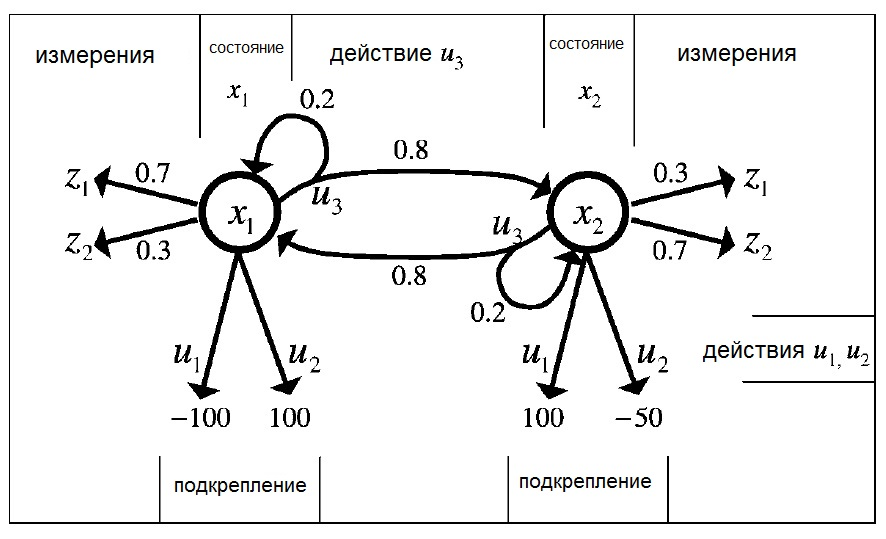
\includegraphics[width=0.8\linewidth]{151orig}}
	\caption{ ( Рис. 15.1 Среда с двумя состояниями, используемая для иллюстрации итерационного алгоритма в пространстве гипотез.) }
	\label{fig:151orig}
\end{figure}

\textbf{15.2	Наглядный пример}\\

\textbf{15.2.1	Исходные данные}\\

Проиллюстрируем итерационный алгоритм в пространствах гипотез с помощью числового примера. Пример является упрощением, но при его обсуждении можно определить все главные элементы итерационного алгоритма в пространствах гипотез.

Рис. 15.1 показана среда с двумя состояниями, обозначенными как $x_1$ и $x_2$. Робот способен выбирать между тремя управляющими действиями, $u_1$, $u_2$ и $u_3$. Действия $u_1$ и $u_2$ окончательны и при их выполнении мгновенно выдаётся следующая награда:\\

(15.4)
$$r(x_1,u_1)=-100\qquad\qquad r(x_2,u_1)=+100$$

(15.5)
$$r(x_1,u_2)=+100\qquad\qquad r(x_2,u_2)=-50$$

Дилемма состоит в том, что оба действия в каждом из состояний дают противоположные награды. В частности, в состоянии $x_1$, оптимальным действием является $u_2$, а действие $u_1$ - в состоянии $x_2$. Таким образом, знание состояния напрямую переносится на награду при выборе оптимального действия.

Чтобы получить такую информацию, у робота есть третье управляющее действие, $u_3$. Выполнение этого действия имеет небольшую стоимость -1:\\

(15.6)
$$r(x_1,u_3)=r(x_2,u_3)=-1$$

Будем считать, что это стоимость ожидания или восприятия. Действие $u_3$ недетерминировано воздействует на состояние среды в:\\

(15.7)
$$p(x_1'|x_1,u_3)=0,2\qquad\qquad p(x_2'|x_1,u_3)=0,8$$

(15.8)
$$p(x_1'|x_2,u_3)=0,8\qquad\qquad p(x_2'|x_2,u_3)=0,2$$

Другими словами, когда робот выполняет действие $u_3$, состояние переключается на противоположное с вероятностью 0,8, а робот платит единичную цену.

Тем не менее, выполнение действия $u_3$ имеет преимущества. Робот может выполнять действие восприятия перед выполнением каждого действия управления. С помощью восприятия робот приобретает знание о состоянии окружающей среды, и, в результате, сможет выбрать лучшее решение управления, которое, в перспективе, даст большую награду. Действие $u_3$ позволяет роботу выполнять восприятие без необходимости выполнения окончательного действия.

В нашем примере модель измерения управляется следующим вероятностным распределением:\\

(15.9)
$$p(z_1|x_1)=0,7\qquad\qquad p(z_2|x_1)=0,3$$

(15.10)
$$p(z_1|x_2)=0,3\qquad\qquad p(z_2|x_2)=0,7$$

Другими словами, если робот выполняет измерение $z_1$, возрастает его уверенность в нахождении в $x_1$, в то же время $z_2$ связано с $x_2$.

Пример с двумя состояниями был выбран потому, что он облегчает изображение функции в пространстве гипотез в виде графика. В частности, гипотеза состояния $b$ характеризуется $p_1 = b(x_1)$ и $p_2 = b(x_2)$. Однако, мы знаем, что $p_2 = 1-p_1$, и этого достаточно для изображения на графике $p_1$. Соответствующая политика управления $\pi$ является функцией, отображающей единичный интервал $[0; 1]$ в пространство всех действий:\\

(15.11)
$$\pi:[0;1]\longrightarrow u$$

\textbf{15.2.2	Выбор управляющего действия}\\

Чтобы определить нужный момент для выполнения управляющего действия, необходимо начать с условия наличия немедленной награды за каждое из трёх управляющих действий, $u_1$, $u_2$ и $u_3$. В предыдущей главе награда считалась функцией состояния и действий.  Поскольку мы не знаем состояния, необходимость поменять выражение для награды, чтобы она соответствовала гипотезе состояния. Таким образом, для любой данный гипотезы $b = (p_1, p_2)$, ожидаемая для этой гипотезы награда задана следующим образом:\\

(15.12)
$$r(b,u)=E_x[r(x,u)]=p_1\,r(x_1,u)+p_2\,r(x_2,u)$$

НАГРАДА в POMDP\\

Функция $r(b, u)$ определяет \textit{награду в POMDP}. 

\begin{figure}[H]
	\center{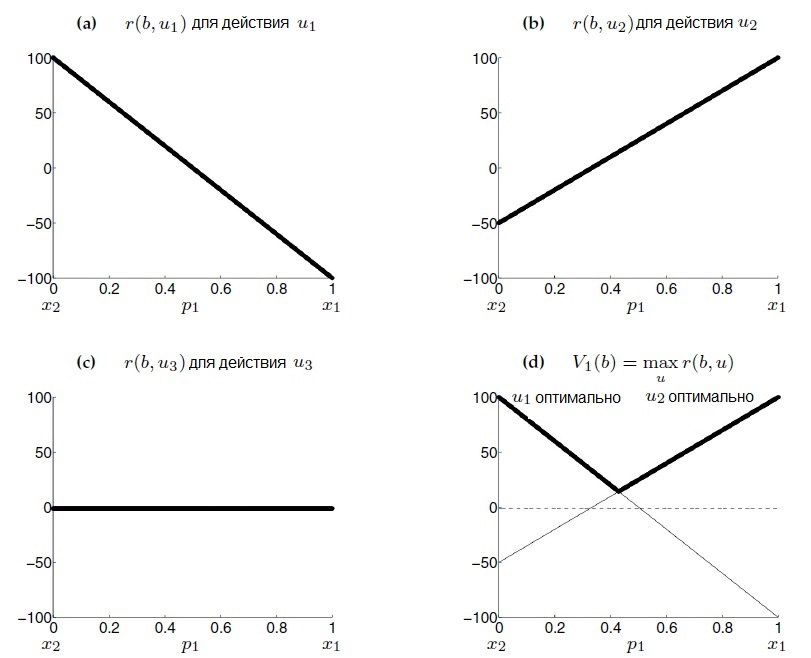
\includegraphics[width=1\linewidth]{152orig}}
	\caption{ ( Рис. 15.2 На схемах (a), (b) и (c) показана ожидаемая награда $r$ в виде функции параметра гипотезы состояния $p_1  =  b(x_1)$ для каждого из трёх действий $u_1$, $u_2$ и  $u_3$.  Функция ценности для горизонта $T = 1$ соответствует максимуму этих трех линейных функций.(d) ) }
	\label{fig:152orig}
\end{figure}

На Рис. 15.2a показаны графики ожидаемой награды $r(b, u_1)$ при выборе управления $u_1$, заданного параметром $p_1$. С левой стороны схемы $p_1 = 0$, и робот абсолютно уверен, что среда находится в состоянии $x_2$. Выполнение действия $u_1$, таким образом, приводит к $r(x_2, u_1) = 100$, как задано в Выражении (15.4). Справа $p_1 = 1$, поэтому состояние $x_1$. Соответственно, выбор элемента управления $u_1$ приведёт к результату $r(x_1, u_1) = -100$. Между тем, функция ожидания даст линейную комбинацию этих двух значений:\\

(15.13)
$$r(b,u_1)=-100p_1+100p_2=-100p_1+100(1-p_1)$$

Эта функция изображена на Рис. 15.2a. 

На Рис.15.2b и (c) показаны соответствующие функции для действия $u_2$ и $u_3$, соответственно. Для $u_2$, получаем \\

(15.14)
$$r(b,u_2)=100p_1-50(1-p_1)$$

а для $u_3$ – постоянную функцию\\

(15.15)
$$r(b,u_3)=-1p_1-1(1-p_1)=-1$$

Первым упражнением будет понимание функции итерационного алгоритма в пространствах гипотез для вычисление функции дохода $V_1$, которая является оптимальной функцией ценности для процессов выбора с горизонтом $T = 1$. В одном цикле выбора робот имеет возможность остановиться на одном из трёх управляющих действий. Так какое следует предпочесть?

Ответ легко прочесть на показанных схемах. Для любой гипотезы состояния $p_1$ на схемах на Рис. 15.2a-c показаны графики ожидаемой награды для каждого выбора действий. Поскольку целью является максимизация награды, робот просто выбирает действие с наивысшим ожиданием награды. Это показано на Рис. 15.2d: на схеме представлены все три графика ожидаемой награды. В левой части оптимальным действием является $u_1$, поскольку преобладает его функция дохода. Переход происходит в момент, когда $r(b, u_1) = r(b, u_2)$, что разрешается до $p_1 = \frac{3}{7}$. Для значений $p_1$ больших, чем $\frac{3}{7}$, $u_2$ будет лучшим выбором. Поэтому, $(T = 1)$-оптимальная политика\\

(15.16)
\begin{equation*}
\pi_1(b)= \left\{
\begin{array}{ll}
u_1& \mbox{ если } p_1 \leq \frac{3}{7} \\
u_2& \mbox{ если } p_1 > \frac{3}{7} 
\end{array}
\right.
\end{equation*}

Соответствующее значение показано жирной линией на графике на Рис. 15.2d. Это график кусочно-линейной выпуклой функции, которая является максимумом отдельных функций награды на Рис. 15.2a-c. Поэтому, можно записать ее в виде максимума трёх функций:\\

(15.17)
\begin{equation*}
\begin{split}
V_1(b)&=\underset{u}{\max}\,r(b,u)\\
&=\max\left\{
\begin{array}{rr}
-100p_1&+100(1-p_1)\\
100p_1&-50(1-p_1)\\
-1&{} 
\end{array}
\right\}\quad
\begin{array}{c}
(\ast)\\(\ast)\\
{}
\end{array}
\end{split}
\end{equation*}

Очевидно, вклад вносят только линейные функции, обозначенные $(\ast)$ в (15.17). Оставшуюся линейную функцию можно смело отбросить:\\

(15.18)
\begin{equation*}
V_1(b)=\max\left\{
\begin{array}{rr}
-100p_1&+100(1-p_1)\\
100p_1&-50(1-p_1)\\
\end{array}
\right\}
\end{equation*}

В рассматриваемом примере мы будем неоднократно использовать прием с обрезкой. Обрезка линейных ограничений показана пунктиром на Рис. 15.2d и многих рисунках в ходе изложения.\\

\textbf{15.2.3	Восприятие}

На следующем шаге добавим восприятие. Что, если робот способен воспринимать среду перед тем, как выполнить выбор действия? Как это повлияет на функцию оптимальной ценности? Очевидно, восприятие даст дополнительную информацию об окружающем мире, позволяя роботу выбрать верное действие. В частности, для наихудшей возможной гипотезы, $p_1 = \frac{3}{7}$, ожидаемая награда в наших примерах составила  $\frac{100}{7}\approx 14,3$, соответствующему значение на перегибе графика на Рис. 15.2d. Очевидно, если бы можно было получить информацию об окружающем, гипотеза бы изменилась. Ценность этой гипотезы будет больше 14,3, но насколько?

Ответ несколько неожиданный. Допустим, результат восприятия $z_1$. На Рис. 15.3a показана гипотеза после восприятия $z_1$ как функция гипотезы до измерения. Давайте проанализируем эту функцию. Если наша гипотеза до восприятия была $p_1 = 0$, гипотеза после измерения останется  $p_1 = 0$, независимо от результатов измерения. Аналогично для $p_1 = 1$. Поэтому, на противоположных концах функция идентична. Но в середине графика имеется неопределённость оценки состояния среды, и процесс измерения $z_1$ смещает гипотезу. Величина смещения регулируется теоремой Байеса:\\

(15.19)
\begin{equation*}
\begin{split}
p_1'&=p(x_1|z)\\
&=\frac{p(z_1|x_1)p(x_1)}{p(z_1)}\\
&=\frac{0,7p_1}{p(z_1)}
\end{split}
\end{equation*}

и\\

(15.20)
\begin{equation*}
p_2'=\frac{0,3(1-p_1)}{p(z_1)}
\end{equation*}

Нормирующий член $p(z_1)$ добавляет нелинейность на Рис. 15.3a. В нашем примере он разрешается до\\

(15.21)
$$p(z_1)=0,7p_1+0,3(1-p_1)=0,4p_1+0,3$$

поэтому $p_1'=\frac{0,7p_1}{0,4p_1+0,3}$.  Однако, как будет показано ниже, этот нормирующий член 
свободно отбрасывается. Подробнее несколько ниже.

Давайте сначала изучим эффект этой  передаточной функции на функцию дохода $V_1$. Допустим, известен результат измерения $z_1$, а затем необходимо сделать выбор действия. Каким будет этот выбор и как будет выглядеть соответствующая функция дохода? Ответ приведён в графическом виде на Рис. 15.3c. На рисунке показана кусочно-линейная функция дохода из Рис. 15.3b, спроектированная с помощью нелинейной функции измерения, обсуждаемой выше (и показанная на Рис. 15.3a). Читателю может понадобится какое-то время, чтобы сориентироваться: Берём гипотезу $p_1$ и проектируем ее на соответствующую гипотезу $p_1'$ согласно нелинейной функции, а затем указываем ее значение на Рис. 15.3b. Эта процедура для всех $p_1\in[0; 1]$, даст график, показанный на Рис. 15.3c.

\begin{figure}[H]
	\center{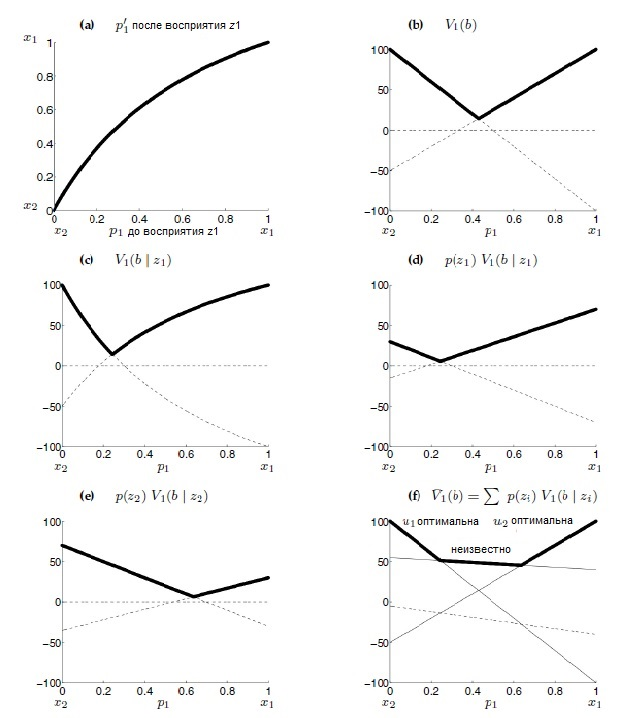
\includegraphics[width=1\linewidth]{153orig}}
	\caption{ ( Рис. 15.3 Эффект восприятия на функцию дохода: (a) Гипотеза после восприятия  $z_1$ как функция гипотезы до восприятия $z_1$. Измерения $z_1$ увеличивает уверенность робота в состоянии $x_1$. Проекция функции дохода на график (b) с помощью этой нелинейной функции даст нелинейную функцию дохода, показанную на (c). (d) деление функции дохода на вероятность наблюдения $z_1$ даст кусочно-линейную функцию. (e) Такая же кусочно-линейная функция для измерения $z_2$. (f) ожидаемая функция дохода после восприятия.) }
	\label{fig:153orig}
\end{figure}

Математически, график задан в виде\\

(15.22)
\begin{equation*}
\begin{split}
V_1(b|z_1)&=\max\left\{
\begin{array}{rr}
-100\cdot\frac{0,7p_1}{p(z_1)}&+100\cdot\frac{0,3(1-p_1)}{p(z_1)}\\
100\cdot\frac{0,7p_1}{p(z_1)}&-50\cdot\frac{0,3(1-p_1)}{p(z_1)} 
\end{array}
\right\}\\
&=\frac{1}{p(z_1)}\max\left\{
\begin{array}{rr}
-70p_1&+30(1-p_1)\\
70p_1&-15(1-p_1)
\end{array}\right\}
\end{split}
\end{equation*}

что является просто результатом замены $p_1$ на $p_1'$ в функции дохода $V_1$ , приведённой в (15.18). Заметим, что на Рис. 15.3c гипотеза «наихудшего» значения смещена влево. Теперь худшая гипотеза - та, которая после восприятия $z_1$, заставляет думать с  вероятностью $\frac{3}{7}$, что робот находится в состоянии $x_1$.

Однако, это соображение касается только одного из двух измерений, а значение до восприятия должно учитывать оба. Значение до восприятия, обозначенное $\bar{V}_1$, задано следующим ожиданием:\\

(15.23)
$$\bar{V}_1(b)=E_z[V_1(b|z)]=\sum_{i=1}^2p(z_i)V_1(b|z_i)$$

Сразу же можно заметить, что в этом ожидании каждая участвующая функция ценности $V_1(b|z_i)$ умножается на вероятность $p(z_i)$, которая была причиной нелинейности для функции ценности до измерения. Вставка (15.19) в это выражение даст\\

(15.24)
\begin{equation*}
\begin{split}
\bar{V}_1(b)&=\sum_{i=1}^2p(z_i)V_1(\frac{p(z_i|x_1)p_1}{p(z_i)})\\
&=\sum_{i=1}^2p(z_i)\frac{1}{p(z_i)}V_1(p(z_i|x_1)p_1)\\
&=\sum_{i=1}^2V_1(p(z_i|x_1)p_1)
\end{split}
\end{equation*}

Эта информация истинна, поскольку каждый элемент в $V_1$ линеен на $1/p(z_i)$, как показано на примере в (15.22). Теперь стало возможно вынести множитель $1/p(z_i)$ из функции максимизации. После решения выражения $p(z_i)$ просто сокращается!

В нашем примере два измерения, поэтому можно вычислить ожидание $p(z_i) V_1(b|z_i)$ для каждого из них. Читатель может вспомнить, что эти ожидания суммировались в выражении (15.23). Для $z_1$ мы уже вычислили $V_1(b|z_i)$ в (15.22), поэтому\\

(15.25)
\begin{equation*}
p(z_1)V_1(b|z_1)=\max\left\{
\begin{array}{rr}
-70p_1&+30(1-p_1)\\
70p_1&-15(1-p_1)\\
\end{array}
\right\}
\end{equation*}

Эта функция показана на Рис. 15.3d и, действительно, является максимумом двух линейных функций. Аналогично, для $z_2$ получаем\\

(15.26)
\begin{equation*}
p(z_2)V_1(b|z_2)=\max\left\{
\begin{array}{rr}
-30p_1&+70(1-p_1)\\
30p_1&-35(1-p_1)\\
\end{array}
\right\}
\end{equation*}

Эта функция приведена на Рис. 15.3e.

Искомая функция дохода до учёта восприятия получается сложением этих двух членов, согласно выражению (15.23):\\

(15.27)
\begin{equation*}
\bar{V}_1=\max\left\{
\begin{array}{rr}
-70p_1&+30(1-p_1)\\
70p_1&-15(1-p_1)\\
\end{array}
\right\}
+\max\left\{
\begin{array}{rr}
-30p_1&+70(1-p_1)\\
30p_1&-35(1-p_1)\\
\end{array}
\right\}
\end{equation*}

Эта сумма показана на Рис. 15.3f. Она имеет примечательную форму: вместо одного перегиба на функции присутствует два, разделяющий функцию ценности на три разных линейных сегментов. Для левого сегмента оптимальным выбором является $u_1$, вне зависимости от информации, которую робот может получить с помощью восприятия. Аналогично для правого сегмента, где оптимальным выбором является $u_2$, вне зависимости от каких-либо обстоятельств. Однако, в центральном секторе восприятие робота имеет значение, определяющее оптимальное действие. В силу этого, в центральном сегменте определяется значение, которое существенно выше, чем соответствующее значение без учёта восприятия, что видно из Рис. 15.2d. Самое главное, что возможность восприятия поднимает значение функции дохода на более высокий уровень в целом регионе, где робот менее уверен в состоянии окружающего мира. Это существенное наблюдение показывает, что что итерационный алгоритм в пространстве гипотез, действительно, зависит от восприятия, но только до тех пор, пока восприятие влияет на выбор действий управления в будущем.

Вернёмся к вычислению функции ценности, поскольку это может оказаться легче, чем ожидалось. Выражение (15.27) требует вычисления суммы двух максимумов линейных функций. Выражение в канонической форме, то есть в виде максимума линейных функций без суммы, потребует некоторых размышлений. В частности, новая функция дохода $\bar{V}_1$ будет ограничена снизу любой суммой, которая добавляет линейную функцию из первого выражения максимизации к линейной функции из второго выражения максимизации. Это даёт четыре возможные комбинации:\\

(15.28)
\begin{equation*}
\begin{split}
\bar{V}_1(b)&=\max\left\{
\begin{array}{rrrr}
-70p_1&+30(1-p_1)&-30p_1&+70(1-p_1)\\
-70p_1&+30(1-p_1)&+30p_1&-35(1-p_1)\\
70p_1&-15(1-p_1)&-30p_1&+70(1-p_1)\\
70p_1&-15(1-p_1)&+30p_1&-35(1-p_1)\\
\end{array}
\right\}\\
&=\max\left\{
\begin{array}{rr}
-100p_1&+100(1-p_1)\\
-40p_1&-5(1-p_1)\\
40p_1&+55(1-p_1)\\
100p_1&-50(1-p_1)\\
\end{array}
\right\}\quad\begin{array}{c}
(\ast)\\
{}\\
(\ast)\\
(\ast)\\
\end{array}\\
&=\max\left\{
\begin{array}{rr}
-100p_1&+100(1-p_1)\\
40p_1&+55(1-p_1)\\
100p_1&-50(1-p_1)\\
\end{array}
\right\}
\end{split}
\end{equation*}

И снова, используем $(\ast)$ для обозначения ограничений, которые действительно вносят вклад в определение функции ценностей. Как показано на Рис. 15.3f, требуется только три из четырёх функций, а четвертую можно смело отсечь.\\

\textbf{15.2.4	Прогнозирование}\\

Финальный этап учитывает переход состояний. Когда робот выполняет действие, его состояние меняется. Для планирования на горизонте глубже $T = 1$, необходимо принимать во внимание и соответствующим образом проектировать функцию дохода. В нашем примере $u_1$ и $u_2$ оба действия окончательными. Теперь осталось только оценить эффект воздействия $u_3$.

К счастью, переходы состояний не всегда так сложны, как измерения в POMDP. На Рис. 15.4a показана проекция гипотезы после выполнения $u_3$. Допустим, робот начинает в состоянии $x_1$ с абсолютной уверенностью, то есть $p_1 = 1$. Затем, согласно модели вероятности перехода в Выражении (15.7),  получим $p_1'  =  p(x_1'|x_1, u_3)=0,2$. Аналогично, для $p_1=0$ получим  $p_1' = p(x_1'|x_2, u_3) = 0,8$. Между этими величинами ожидание линейно:\\

(15.29)
\begin{equation*}
\begin{split}
p_1'&=E_x[p(x_1'|x,u_3)]\\
&=\sum_{i=1}^2 p(x_1'|x_i,u_3)p_i\\
&=0,2p_1+0,8(1-p_1)=0,8-0,6p_1
\end{split}
\end{equation*}

Эта функция графически представлена на Рис. 15.4a. Если теперь отобразить функцию ценности на Рис. 15.4b (что эквивалентно функции, показанной на Рис. 15.3f), мы получим функцию ценности на Рис. 15.4c. Эта функция ценности более плоская, чем та, что была до проекции, выражая потерю информации из-за смены состояний. Она также отражена зеркально, поскольку ожидание состояния изменяется при выполнении $u_3$.

\begin{figure}[H]
	\center{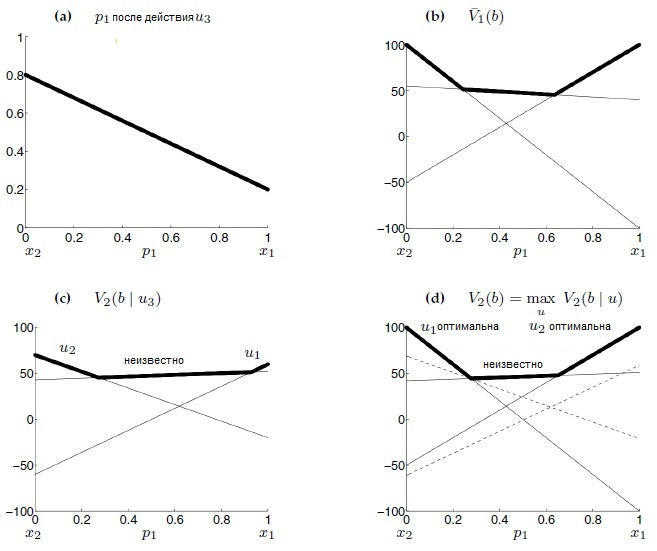
\includegraphics[width=1\linewidth]{154orig}}
	\caption{ ( Рис. 15.4  (a) Параметр гипотезы состояния $p_1'$  после выполнения действия $u_3$, как функция параметра $p_1$ до выполнения действия. Распространение гипотезы показано на схеме (b) с помощью инверсии результатов проекции гипотезы, показанной на (c). (d) Функция дохода $V_2$ получена максимизацией функции гипотезы после ее прохождения, и награды двух оставшихся действий, $u_1$ и $u_2$.) }
	\label{fig:154orig}
\end{figure}

Математически, эта функция ценности вычисляется проектированием (15.28) через (15.29).\\

(15.30)
\begin{equation*}
\begin{split}
\bar{V}_1(b|u_3)&=\max\left\{
\begin{array}{rr}
-100(0,8-0,6p_1)&+100(1-(0,8-0,6p_1))\\
40(0,8-0,6p_1)&+55(1-(0,8-0,6p_1))\\
100(0,8-0,6p_1)&-50(1-(0,8-0,6p_1))\\
\end{array}
\right\}\\
&=\max\left\{
\begin{array}{rr}
-100(0,8-0,6p_1)&+100(0,2+0,6p_1)\\
40(0,8-0,6p_1)&+55(0,2+0,6p_1)\\
100(0,8-0,6p_1)&-50(0,2+0,6p_1)\\
\end{array}
\right\}\\
&=\max\left\{
\begin{array}{rr}
60p_1&-60(1-p_1)\\
52p_1&+43(1-p_1)\\
-20p_1&+70(1-p_1)\\
\end{array}
\right\}
\end{split}
\end{equation*}

Эти преобразования легко проверить вручную. Такая функция вместе с оптимальными управляющими действиями показаны на Рис. 15.4c.

Теперь конструирование функции дохода $V_2$ с горизонтом планирования $T = 2$ почти завершено. И снова перед роботом стоит выбор, выполнить ли действие $u_3$, или же одно из окончательных действий $u_1$ или $u_2$. Как и прежде, этот выбор выполняется дополнением в набор условий двух новых вариантов в виде двух линейных функций $r(b, u_1)$ и $r(b, u_2)$. Мы также должны вычесть стоимость выполнения действия $u_3$ из функции ценности.

Это даст схему, изображённую на Рис. 15.4d, которая имеет вид\\

(15.31)
\begin{equation*}
\bar{V}_2(b)=\max\left\{
\begin{array}{rr}
-100p_1&+100(1-p_1)\\
100p_1&-50(1-p_1)\\
59p_1&-61(1-p_1)\\
51p_1&+42(1-p_1)\\
-21p_1&+69(1-p_1)\\
\end{array}
\right\}\quad
\begin{array}{c}
(\ast)\\(\ast)\\{}\\(\ast)\\{}
\end{array}
\end{equation*}

Заметим, что было просто добавлено два варианта (строки один и два), и выполнено вычитание равномерной стоимости $u_3$ из всех других линейных ограничений (строки с третьей по пятую). И снова, необходимы только три из этих ограничений, обозначенных $(\ast)$. Результирующее значение может быть переписано в виде\\

(15.32)
\begin{equation*}
\bar{V}_2(b)=\max\left\{
\begin{array}{rr}
-100p_1&+100(1-p_1)\\
100p_1&-50(1-p_1)\\
51p_1&+42(1-p_1)\\
\end{array}
\right\}
\end{equation*}

\begin{figure}[H]
	\center{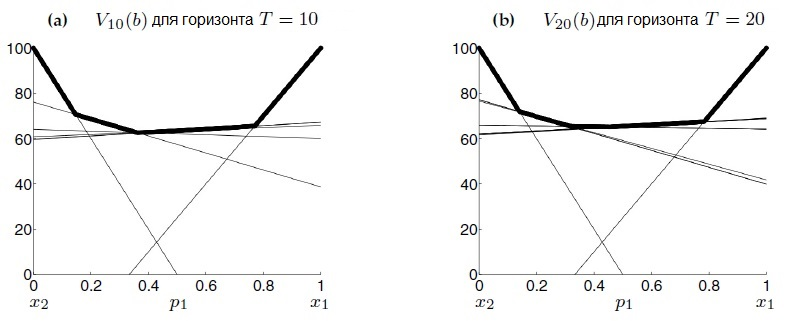
\includegraphics[width=1\linewidth]{155orig}}
	\caption{ ( Рис. 15.5 Функция ценности $V$ для горизонтов $T = 10$ и $T = 20$. Заметим, что масштаб по вертикальной оси на этих графиках отличает от предыдущих графиков функции ценности.) }
	\label{fig:155orig}
\end{figure}

\textbf{15.2.5	Глубокие горизонты и отсекание}\\

ОБРАТНЫЙ ШАГ В ПРОСТРАНСТВЕ ГИПОТЕЗ\\

Мы выполнили полный обратный шаг в пространстве гипотез. Этот алгоритм легко выполняется рекурсивно.
На Рис. 15.5 показана функция дохода для горизонтов $T = 10$ и $T = 20$, соответственно. Обе функции дохода выглядят похоже. С соответствующим отсеканием, в $V_{20}$ имеется только 13 компонент\\

(15.33)
\begin{equation*}
\bar{V}_{20}(b)=\max\left\{
\begin{array}{rr}
-100p_1&+100(1-p_1)\\
100p_1&-50(1-p_1)\\
64,1512p_1&+65,9454(1-p_1)\\
64,1513p_1&+65,9454(1-p_1)\\
64,1531p_1&+65,9442(1-p_1)\\
68,7968p_1&+62,0658(1-p_1)\\
68,7968p_1&+62,0658(1-p_1)\\
69,0914p_1&+61,5714(1-p_1)\\
68,8167p_1&+62,0439(1-p_1)\\
69,0369p_1&+61,6779(1-p_1)\\
41,7249p_1&+76,5944(1-p_1)\\
39,8427p_1&+77,1759(1-p_1)\\
39,8334p_1&+77,1786(1-p_1)\\
\end{array}
\right\}
\end{equation*}

Сверху можно увидеть две уже знакомые функции. Все остальные соответствуют специфическим последовательностям измерений и выбора действий.

Этот простой пример показывает важность отсечения. Без него каждое новое обновление добавляет ещё два линейных ограничения (выбор действий), а затем возводит в квадрат количество ограничений (измерение). Поэтому, значение функции без отсечения  для $T = 20$ определяется по $10^{547864}$ линейным ограничениям, а для $T = 30$ - по $10^{561012337}$. Обрезанная функция дохода, для сравнения, содержит всего 13 таких ограничений.

Этот невероятный взрывной рост является ключевой причиной непрактичности использования простых алгоритмов POMDP. На Рис. 15.6 приводится пошаговое сравнение этапов, которые приводят к функции дохода $V_2$. В левой части показаны функции после отсечения, в правой – все линейные функции. Хотя в этом вычислении всего один шаг измерения, количество неиспользуемых функций уже достаточно велико. Мы вернёмся к этой теме позже, при выводе эффективных приближенных алгоритмов POMDP.

Последним наблюдением в нашем анализе является то, что оптимальная функция дохода для любого конечного горизонта непрерывная, кусочно-линейная и выпуклая. Каждый линейный участок соответствует разному выбору действий в некоторой точке в будущем. Выпуклость функции дохода указывает на довольно очевидное наблюдение, о том, что знание всегда лучше неведения. Если даны две гипотезы состояния $b$ и $b'$, смешанное значение гипотезы состояний больше или равно значению смешанной оценки состояния для некоторого параметра смешивания $\beta$, где $0\leq\beta\leq1$:\\

(15.34)
$$\beta V(b)+(1-\beta)V(b')\geq V(\beta b+(1-\beta)b')$$

Эта формализация применима только для случая конечных горизонтов. Для бесконечного горизонта функция ценности может быть прерывистой и нелинейной.\\

\begin{figure}[H]
	\center{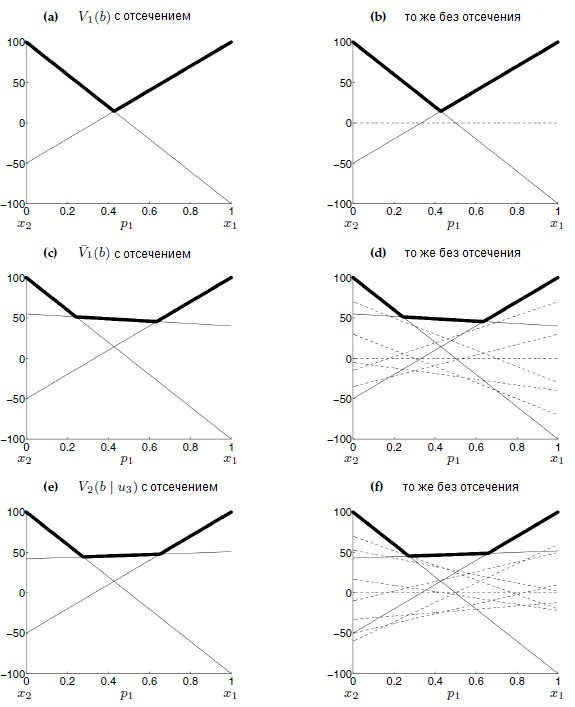
\includegraphics[width=0.9\linewidth]{156orig}}
	\caption{ ( Рис. 15.6 сравнения точного алгоритма отсечения (левый столбец) с алгоритмом POMDP без обрезки (правый столбец), для первых нескольких шагов алгоритма планирования POMDP. Очевидно, количество линейных ограничений существенно увеличивается без отсечения. При $T = 20$ значение функции без обрезки определено $10^{547864}$ линейными функциями, а с обрезкой - всего тринадцатью. ) }
	\label{fig:156orig}
\end{figure}

\textbf{15.3	Алгоритм POMDP для конечной среды}\\

В предыдущем разделе было показано на примере, как вычисляются функции ценности для конечных сред. Здесь мы кратко обсудим общий алгоритм для вычисления функции ценности, перед тем, как вывести его из общих положений.

Алгоритм POMDP приведён в Таблице 15.1. Он принимает на вход единственный параметр $T$, горизонт планирования для POMDP, и возвращает набор векторов параметров, каждый в виде\\

(15.35)
$$(v_1,...,v_N)$$

Каждый из этих параметров определяет линейную функцию в пространстве гипотез вида\\

(15.36)
$$\sum_iv_ip_i$$

МАКСИМУМ ЛИНЕЙНЫХ ФУНКЦИЙ\\

Фактическое значение определяется \textit{максимумом всех этих линейных функций}:\\

(15.37)
$$\underset{(p_1,...,p_N)}{\max}\sum_iv_ip_i$$

Алгоритм POMDP рекурсивно вычисляет значение функций. Начальный набор для псевдо-горизонта $T = 0$ устанавливается в строке 2 Таблицы 15.1. Затем алгоритм POMDP рекурсивно вычисляет новый набор во вложенном цикле в строках 3-24. Ключевые вычисления выполняются в строке 9:  Здесь вычисляются коэффициенты линейных функций $v_{u,z,j}^k$, необходимые для следующего набора линейных ограничений.
Каждая линейная функция возникает из выполнения управляющего действия $u$, за которым следует измерение восприятия $z$, и выполнение действия управления $u'$. Линейное ограничение, соответствующее $u'$, было вычислено в предыдущей итерации для меньшего горизонта планирования (взятого в строке 5). Поэтому, по достижении строки 14, была сгенерирована одна линейная функция для каждой комбинации действия управления, измерения и линейного ограничения предыдущей функции ценности.

Линейные ограничения новой функции дохода вычисляются взятием ожиданий по измерениям, как это сделано в строках 14-21. Для каждого действия управления алгоритм в строке 15 генерирует $K^M$ таких линейных ограничений. Такое большое количество возникает из-за того, что каждое ожидание берётся по $M$ возможным измерениям, каждое из которых можно «комбинировать» с любым из $K$ ограничений, содержащихся в предыдущей функции значимости. В строке 17 вычисляется ожидание для каждой из таких комбинаций. Результирующее ограничение добавляется к новому набору ограничений в строке 19.\\

\begin{table}[H]
\begin{center}
\begin{tabular}{|l|}
\hline
{}\\
1:\textbf{ Algorithm POMDP}$(T):$\\
2:\hspace{5mm}$\varUpsilon=(0;0,...,0)$\\
3:\hspace{5mm}$\textit{for}\,\tau=1\,\textit{to}\,T\,\textit{do}$\\
4:\hspace{10mm}$\varUpsilon'=\emptyset$\\
5:\hspace{10mm}$\textit{для всех}\,(u';v_1^k,...v_N^k)\,\textit{в}\,\varUpsilon\,\textit{выполнить}$\\
6:\hspace{15mm}$\textit{для всех управляющих действий u выполнить}$\\
7:\hspace{20mm}$\textit{для всех измеренийs z выполнить}$\\
8:\hspace{25mm}$\textit{for}\,j=1\,\textit{to}\,N\,\textit{do}$\\
9:\hspace{30mm}$v_{u,z,j}^k=\sum_{i=1}^Nv_i^kp(z|x_i)p(x_i|u,x_j)$\\
10:\hspace{24mm}$\textit{endfor}$\\
11:\hspace{19mm}$\textit{endfor}$\\
12:\hspace{14mm}$\textit{endfor}$\\
13:\hspace{9mm}$\textit{endfor}$\\
14:\hspace{9mm}$\textit{для всех управляющих действий u выполнить}$\\
15:\hspace{14mm}$\textit{для всех}\,k(1),...,k(M)=(1,...,1)\,\textit{to}\,(|\varUpsilon|,...,|\varUpsilon|)\,\textit{выполнить}\qquad\qquad$\\
16:\hspace{19mm}$\textit{для}\,i=1\,\textit{до}\,N\,\textit{выполнить}$\\
17:\hspace{24mm}$v_i'=\gamma[r(x_i,u)+\sum_zv_{u,z,i}^{k(z)}]$\\
18:\hspace{19mm}$\textit{endfor}$\\
19:\hspace{19mm}$\textit{прибавить}\,(u;v_1',...,v_N')\,\textit{к}\,\varUpsilon'$\\
20:\hspace{14mm}$\textit{endfor}$\\
21:\hspace{9mm}$\textit{endfor}$\\
22:\hspace{9mm}$\textit{опционально:\,обрезать}\,\,\varUpsilon'$\\
23:\hspace{9mm}$\varUpsilon=\varUpsilon'$\\
24:\hspace{5mm}$\textit{endfor}$\\
25:\hspace{5mm}$\textit{return}\,\,\varUpsilon$\\
{}\\
\hline
\end{tabular}
\caption{(Таблица 15.1 Алгоритм POMDP для дискретных сред. Этот алгоритм выражает оптимальную функцию значимости в виде набора вычисляемых рекурсивно линейных ограничений.)}
\end{center}
\end{table}

\begin{table}[H]
\begin{center}
\begin{tabular}{|l|}
\hline
{}\\
1:\textbf{ Algorithm policy POMDP}$(\varUpsilon,b=(p_1,...,p_N)):\qquad\qquad\qquad$\\
2:\hspace{5mm}$\hat{u}=\underset{(u;v_1^k,...,v_N^k)}{\text{argmax}}\sum_{i=1}^Nv_i^kp_i$\\
3:\hspace{5mm}$\textit{return}\,\,\hat{u}$\\
{}\\
\hline
\end{tabular}
\caption{(Таблица 15.2 Алгоритм определения оптимального действия для политики, выраженной набором линейных функций $\varUpsilon$.)}
\end{center}
\end{table}

Алгоритм для нахождения оптимального управляющего действия показан в Таблице 15.2. На вход алгоритма поступает гипотеза состояния, заданная в виде $b = (p_1,..., p_N)$, а также набор линейных функций $\varUpsilon$. Оптимальное действие определяется поиском по всем линейным функциям, и нахождением той, которая имеет максимальное значение для $b$. Это значение возвращается в строке 3 алгоритма \textbf{policy\_POMDP} в Таблице 15.2.\\

\textbf{15.4	Математический вывод POMDP}\\

\textbf{15.4.1	Итерационный алгоритм в пространстве гипотез}\\

Общее обновление функции дохода выполняется в (15.2), приводится здесь для удобства.\\

(15.38)
$$V_T(b)=\gamma\,\underset{u}{\max}\left[ r(b,u)+\int V_{T-1}(b')p(b'|u,b)db'\right] $$

Начнём с преобразования этого равенства в более практичный вид, чтобы избежать интегрирования по пространству всех возможных гипотез.

Ключевым фактором этого обновления является условная вероятность $p(b' | u, b)$. Она определяет конкретное распределение из множества распределений на основании данных гипотез $b$ и действий управления $u$. Это необходимо потому, что конкретная гипотеза $b'$ также основана на следующем измерении, а само измерение генерируется стохастически. Необходимость иметь дело с распределениями из распределений добавляет излишнюю сложность.

Если зафиксировать измерение, апостериорная оценка $b'$ будет уникальна, а вероятность $p(b' | u, b)$ вырождается до точечного распределения. Почему так? Ответ даст байесовский фильтр. Из гипотезы $b$ перед выполнением действия $u$, и последующего наблюдения $z$, байесовский фильтр вычисляет единственную апостериорную оценку $b'$ которая является единственной и верной гипотезой. Поэтому, можно заключить, что знание $z$, устраняет необходимость интегрирования по всем гипотезам в (15.38).

Эту идею можно использовать, переписав выражение\\

(15.39)
$$p(b'|u,b)=\int p(b'|u,b,z)p(z|u,b)dz$$

где $p(b' | u, b, z)$ - точечное распределение из единственной гипотезы, вычисленной байесовским фильтром. Вставка этого интеграла в Уравнение (15.38) даёт\\

(15.40)
$$V_T(b)=\gamma\,\underset{u}{\max}\left[ r(b,u)+\int\left[ \int V_{T-1}(b')p(b'|u,b,z)db'\right] p(z|u,b)dz\right] $$

Внутренний интеграл\\

(15.41)
$$\int V_{T-1}(b')p(b'|u,b,z)db'$$

содержит только один ненулевой член. Этот член $b'$ является распределением, вычисленным из $b$, $u$, и $z$ с помощью байесовского фильтра. Назовём это распределение $B(b, u, z)$:\\

(15.42)
\begin{equation*}
\begin{split}
B(b,u,z)(x')&=p(x'|z,u,b)\\
&=\frac{p(z|x',u,b)p(x'|u,b)}{p(z|u,b)}\\
&=\frac{1}{p(z|u,b)}p(z|x')\int p(x'|u,b,s)p(x|u,b)dx\\
&=\frac{1}{p(z|u,b)}p(z|x')\int p(x'|u,x)b(x)dx
\end{split}
\end{equation*}

Читатель должен помнить знакомый уже вывод байесовского фильтра, который подробно обсуждался в Главе 2, на этот раз с нормирующим членом в явном виде.

Теперь можно переписать (15.40) в следующем виде. Заметим, что это выражение больше не интегрируется по $b'$.\\

(15.43)
$$V_T(b)=\gamma\,\underset{u}{\max}\left[ r(b,u)+\int V_{T-1}(B(b,u,z))p(z|u,b)dz\right] $$

Эта форма более удобна по сравнению с первоначальной в (15.38), поскольку требует интегрирования по всем возможным измерениям $z$, вместо всех возможных распределений гипотез $b'$. Это преобразование было косвенно использовано в примере выше, где новая функция ценности получалась путём смешивания конечного множества кусочно-линейных функций.

Дальше будет удобнее отделить максимизацию по действиям от интегрирования. Далее, заметим, что (15.43) можно переписать в виде двух равенств:\\

(15.44)
$$V_T(b,u)=\gamma\,\left[ r(b,u)+\int V_{T-1}(B(b,u,z))p(z|u,b)dz\right] $$

(15.45)
$$V_T(b)=\underset{u}{\max}V_T(b,u)$$

Здесь $V_T (b, u)$ - горизонт $T$ –функции дохода по гипотезе $b$, считая, что следующее действие $u$.

\textbf{15.4.2	Выражение функции дохода}\\

Как и в примере, выразим функцию дохода в виде максимума набора линейных функций.  Мы уже обсуждали, что любая линейная функция по одиночной гипотезе может быть выражено набором коэффициентов $v_1,..., v_N$:\\

(15.46)
$$V(b)=\sum_{i=1}^N v_ip_i$$

где, как обычно, $p_1,..., p_N$ параметры распределения гипотез $b$. Как и в примере, кусочно-линейная выпуклая функция $V_T (b)$ может быть выражена в виде максимума конечного набора линейных функций\\

(15.47)
$$V(b)=\underset{k}{\max}\sum_{i=1}^N v_i^k p_i$$

где $v_1^k,..., v_N^k$ означает параметры $k$-й линейной функции. Читатель должен быстро убедиться, что максимум конечного набора линейных функций действительно выпуклая, непрерывная и кусочно-линейная функция.\\

\textbf{15.4.3	Вычисление функции дохода}\\

Выведем рекурсивное выражение для вычисления функции дохода $V_T (b)$. Исходя из соображений индукции, что $V_{T-1}(b)$, функция ценности для горизонта $T-1$, выраженная кусочно-линейной функцией как указывалось выше. Как часть вывода, продемонстрируем, что при допущении, что $V_{T-1}(b)$ является кусочно-линейной и выпуклой, $V_T (b)$ также кусочно-линейная и выпуклая. Индукция по горизонту планирования $T$ доказывает, что все функции дохода с конечным горизонтом, действительно, кусочно-линейные и выпуклые.

Начнём с выражений (15.44) и (15.45). Если пространство измерений конечно, можно заменить интегрирование по $z$ конечной суммой.\\

(15.48)
$$V_T(b,u)=\gamma\,\left[ r(b,u)+\sum_z V_{T-1}(B(b,u,z))p(z|u,b)\right] $$

(15.49)
$$V_T(b)=\underset{u}{\max}V_T(b,u)$$

Гипотеза $B(b, u, z)$ получается, используя следующее выражение, выведенное из выражения (15.42) заменой интеграла конечной суммой.\\

(15.50)
$$B(b,u,z)(x')=\frac{1}{p(z|u,b)}p(z|x')\sum_xp(x'|u,x)b(x)$$

Если гипотеза $b$ выражена параметрами $\{p_1,..., p_N \}$, а гипотеза
$B(b, u, z)$ - параметрами $\{p_1',..., p_N'\}$, следовательно $j$-й параметр гипотезы $b'$ вычисляется следующим образом:\\

(15.51)
$$p_j'=\frac{1}{p(z|u,b)}p(z|x_j)\sum_{i=1}^Np(x_j|u,x_i)p_i$$

Для вычисления обновления функции ценности (15.48), найдём более практичное выражение для члена $V_{T-1}(B(b, u, z))$, используя описанные выше конечные суммы. Наш вывод начинается с определения $V_{T-1}$ и замены $p_j'$ в соответствии с выражением (15.51):\\

(15.52)
\begin{equation*}
\begin{split}
V_{T-1}(B(b,u,z))&=\underset{k}{\max}\sum_{j=1}^N v_j^k p_j'\\
&=\underset{k}{\max}\sum_{j=1}^N v_j^k \frac{1}{p(z|u,b)}p(z|x_j)\sum_{i=1}^Np(x_j|u,x_i)p_i\\
&=\frac{1}{p(z|u,b)}\underset{k}{\max}\sum_{j=1}^N v_j^kp(z|x_j)\sum_{i=1}^Np(x_j|u,x_i)p_i\\
&=\frac{1}{p(z|u,b)}\underset{k}{\max}\overbrace{\sum_{i=1}^Np_i\underbrace{\sum_{j=1}^N v_j^kp(z|x_j)p(x_j|u,x_i)}_{(\ast)}}^{(\ast\ast)}
\end{split}
\end{equation*}

Член гипотезы, обозначенный $(\ast)$ независим. Поэтому, функция, обозначенная $(\ast\ast)$ является линейной функцией в параметрах пространства гипотез, $p_1,..., p_N$ . Член $1/p(z | u, b)$ нелинейный и трудно вычисляется, поскольку содержит полную гипотезу $b$ как условную переменную. Однако, красота POMDP состоит в том, что это выражение можно отбросить. В частности, замена этого выражения обратно в  (15.48) даст следующее равенство обновления:\\

(15.53)
$$V_T(b,u)=\gamma\,\left[ r(b,u)+\sum_z\underset{k}{\max}\sum_{i=1}^Np_i\sum_{j=1}^Nv_j^kp(z|x_j)p(x_j|u,x_i)\right] $$

Поэтому, несмотря на нелинейность, возникающую при обновлении измерения, $V_T (b, u)$ тоже кусочно-линейная функция.

Наконец, заметим, что $r(b, u)$ задан ожиданием\\

(15.54)
$$r(b,u)=E_x[r(x,u)]=\sum_{i=1}^Np_ir(x_i,u)$$

Здесь подразумевается, что гипотеза $b$ выражена параметрами
$\{p_1,..., p_N \}$.

Искомая функция ценности $V_T$  теперь получается максимизацией $V_T(b, u)$
по всем действиям $u$, как показано в (15.49):\\

(15.55)
\begin{equation*}
\begin{split}
V_T(b)&=\underset{u}{\max}V_T(b,u)\\
&=\gamma\,\underset{u}{\max}\left( \left[ \sum_{i=1}^N p_ir(x_i,u)\right]+ \sum_z\underset{k}{\max}\sum_{i=1}^Np_i\underbrace{\sum_{j=1}^N v_j^kp(z|x_j)p(x_j|u,x_i)}_{=:v_{u,z,i}^k} \right)   \\
&=\gamma\,\underset{u}{\max}\left( \left[ \sum_{i=1}^N p_ir(x_i,u)\right]+\underbrace{\sum_z\underset{k}{\max}\sum_{i=1}^N p_iv_{u,z,i}^k}_{(\ast)}\right) 
\end{split}
\end{equation*}

где

(15.56)
$$v_{u,z,i}^k=\sum_{j=1}^N v_j^kp(z|x_j)p(x_j|u,x_i)$$

как было показано. Но выражение пока ещё не задано в виде максимума линейных функций. В частности, понадобится поменять выражение «сумма-максимум-сумма», обозначенное $(\ast)$ в (15.55) на выражение вида «максимум-сумма-сумма», которое является максимумом по множеству линейных функций.

Используется то же самое преобразование, которое уже было показано в примере в подразделе 15.2.3.
А именно, допустим, требуется вычислить максимум\\

(15.57)
$$\max\{a_1(x),...,a_n(x)\}+\max\{b_1(x),...,b_n(x)\}$$ 

для некоторых функций $a_1(x),...,a_n(x)$ и $b_1(x),...,b_n(x)$ по переменной $x$.
Максимум получается в виде\\

(15.58)
$$\underset{i}{\max}\,\,\underset{j}{\max}\,[a_i(x)+b_j(x)]$$

Это следует из того факта, что $a_i + b_j$, в действительности, нижняя граница. Далее, для каждого $x$ должны существовать такие $i$ и $j$, что $a_i(x)+b_j(x)$ определяет максимум. Включая все такие потенциальные пары в (15.58) получим плотную нижнюю границу, то есть решение.

Теперь легко выполнить обобщение на произвольные суммы по выражениям максимума:\\

(15.59)
$$\sum_{j=1}^m\,\underset{i=1}{\overset{N}{\max}}\,a_{i,j}(x)=\underset{i(1)=1}{\overset{N}{\max}}\,\underset{i(2)=1}{\overset{N}{\max}}\,...\,\underset{i(m)=1}{\overset{N}{\max}}\sum_{j=1}^ma_{i(j),j}$$

и применить этот приём к вычислению функции дохода POMDP, выразив $(\ast)$ в (15.55). Пусть $M$ будет общим количеством измерений.\\

(15.60)
\begin{equation*}
\begin{split}
\sum_z\underset{k}{\max}\sum_{i=1}^Np_iv_{u,z,i}^k&=\underset{k(1)}{\max}\,\underset{k(2)}{\max}\,...\,\underset{k(M)}{\max}\sum_z\sum_{i=1}^Np_iv_{u,z,i}^{k(z)}\\
&=\underset{k(1)}{\max}\,\underset{k(2)}{\max}\,...\,\underset{k(M)}{\max}\sum_{i=1}^Np_i\sum_zv_{u,z,i}^{k(z)}
\end{split}
\end{equation*}

Здесь каждая $k( )$ является отдельной переменной, каждая из которых принимает значения $k$ с левой стороны знака равенства. Этих переменных столько же, сколько измерений. В результате, искомая функция ценности теперь получается следующим образом:\\

(15.61)
\begin{equation*}
\begin{split}
V_T(b)&=\gamma\,\underset{u}{\max}\left[ \sum_{i=1}^Np_i\,r(x_i,u)\right] +\underset{k(1)}{\max}\,\underset{k(2)}{\max}\,...\,\underset{k(M)}{\max}\sum_{i=1}^Np_i\sum_zv_{u,z,i}^{k(z)}\\
&=\gamma\,\underset{u}{\max}\,\underset{k(1)}{\max}\,\underset{k(2)}{\max}\,...\,\underset{k(M)}{\max}\sum_{i=1}^Np_i\left[ r(x_i,u)+\sum_zv_{u,z,i}^{k(z)}\right] 
\end{split}
\end{equation*}

Другими словами, каждая комбинация\\

$$\left( \left[r(x_1,u)+\sum_zv_{u,z,1}^{k(z)}\right] \,\left[r(x_2,u)+\sum_zv_{u,z,2}^{k(z)}\right]\,...\,\left[r(x_N,u)+\sum_zv_{u,z,N}^{k(z)}\right]\right) $$ 

образует новое линейное ограничение в функции ценности $V_T$.

Для каждого уникального объединённого множества переменных $k(1), k(2),... , k(M)$ будет по одному такому ограничению. Очевидно, максимум этих линейных функций снова кусочно-линейный и выпуклый, что доказывает, что этого выражения достаточно для выражения верной функции ценности по базовому непрерывному пространству гипотез. Далее, количество линейных участков будет дважды экспоненциально относительно пространства измерений, по крайней мере, для нашей наивной реализации, которая сохраняет все такие ограничения.\\

\textbf{15.4	Практические соображения}\\

\begin{figure}[H]
	\center{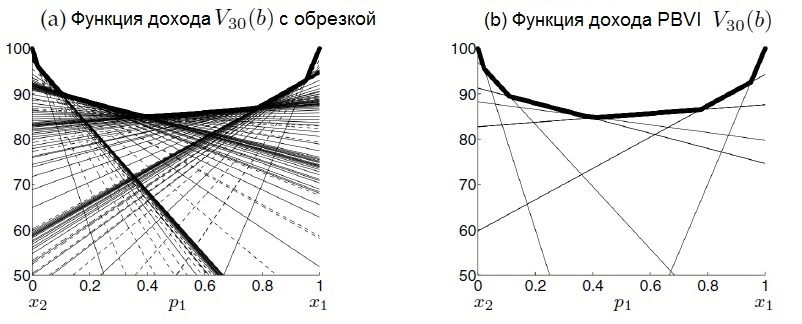
\includegraphics[width=1\linewidth]{157orig}}
	\caption{ ( Рис. 15.7 Преимущества итерационного алгоритма на основе точек над общим итерационным алгоритмом: На схеме (a) показано точное значение функции для горизонта $T = 30$ для другого примера, состоящего из 120 ограничений после отсечения. С правой стороны результат работы алгоритма PBVI сохраняющего только 11 линейных функций. Результаты обоих функции, в части применимости к управлению, практически неразличимы.) }
	\label{fig:157orig}
\end{figure}

Пока что обсуждаемый  итерационный алгоритм далёк от практического. Для любого разумного количества явных состояний, измерений и действий управления сложность функции дохода чрезмерная, даже при относительно небольших горизонтах планирования.

Существует ряд возможностей реализовать более эффективные алгоритмы. Одна такая возможность уже обсуждалась в примере: количество линейных ограничений быстро растет до чрезмерных значений. К счастью, большое количество линейных ограничений можно смело игнорировать, поскольку они не участвуют в определении максимума.

Другим связанным недостатком  итерационного алгоритма является вычисление функций дохода \textit{для всех} гипотез состояния, не только для релевантных. Когда робот начинает с хорошо определённой гипотезой состояния, набор доступных гипотез состояния часто достаточно мал. Например, если робот пытается пройти через две двери, для которых неизвестно, открыты они или закрыты, состояние первой двери станет очевидным при достижении второй. Поэтому, гипотеза состояния, в которой известно только состояние второй двери, когда первой – неизвестно, физически невозможно. Во многих областях применения недостижимы огромные участки пространства гипотез.

Даже для достижимых гипотез некоторые могут быть достижимы лишь с малой вероятностью. Другие могут быть просто нежелательны, и робот будет избегать их. Итерационный алгоритм таких различий не делает. Фактически, время и ресурсы, вложенные в вычисления дохода, не зависят от шансов релевантности гипотезы состояния.

\begin{figure}[H]
	\center{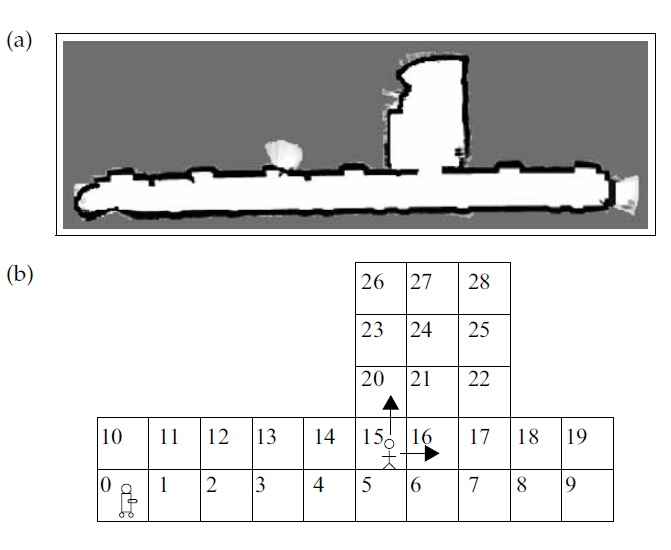
\includegraphics[width=0.9\linewidth]{158orig}}
	\caption{ ( Рис. 15.8 Среда внутри помещения, в которой выполняется поиск политики обнаружения движущегося нарушителя.  Карта сетки занятости(a), и  дискретное пространство состояния POMDP (b). Робот отслеживает своё положение достаточно хорошо, чтобы игнорировать неопределенность положения. Оставшаяся неопределенность относится к местоположению человека. Собственность Джолли Пиню, университет МакГилла (Joelle Pineau, McGill University).) }
	\label{fig:158orig}
\end{figure}

ИТЕРАЦИОННЫЙ АЛГОРИТМ НА ОСНОВЕ ТОЧЕК\\

Существует огромное множество алгоритмов, которые более разборчивы относительно областей пространства гипотез, для которых вычисляется функция дохода. Один из них называется итерационный алгоритм на основе точек \textit{(point-based value iteration – PBVI)} и основан на идее сохранения набора эталонных гипотез состояний, и ограничения функции дохода лишь теми ограничениями, которые максимизируют её значение для, по крайней мере, одной из этих гипотез состояний. Представим, что дано множество гипотез состояния $B = {b_1, b_2,...}$, называемых \textit{точками гипотез}. Затем, \textit{приведённая функция дохода} $V$ по отношению к $B$ является набором ограничений $v\in V$  для которого можно найти, по крайней мере, один $b_i\in B$ такой, чтобы $v(b_i)=V(b_i)$.  Другими словами, линейные сегменты, которые не совпадают с какой-либо дискретной точкой гипотезы в $B$, отбрасываются. Оригинальный алгоритм PBVI эффективно вычисляет функцию дохода даже не генерируя ограничения, которые не поддерживаются какой-либо из точек. Однако, та же самая идея может быть реализована отсечением всех линейных сегментов после их генерации в стандартном обратном шаге POMDP.

\begin{figure}[H]
	\center{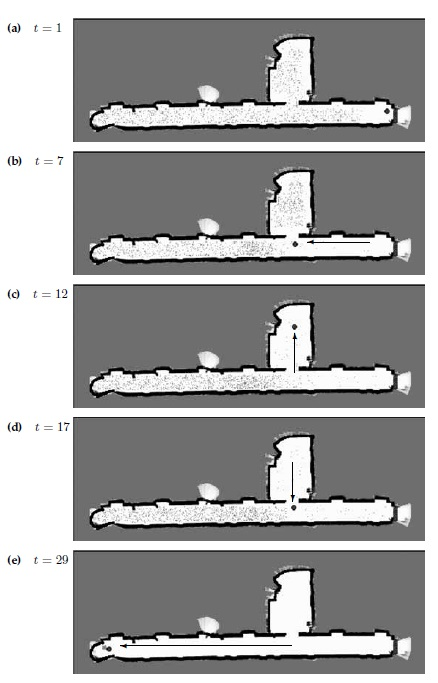
\includegraphics[width=0.95\linewidth]{159orig}}
	\caption{ ( Рис. 15.9 Успешная политика поиска. Здесь отслеживание нарушителя реализовано с помощью многочастичного фильтра, который затем проектируется на выражение в виде гистограммы, подходящее для POMDP. Робот сначала осматривает комнату сверху, а затем проходит ниже по коридору. Собственность Джоелли Пиню, университет МакГилла (Joelle Pineau, McGill University). ) }
	\label{fig:159orig}
\end{figure}

Идея сохранения множества точек гипотез может существенно улучшить эффективность итерационного алгоритма. На Рис. 15.7a показана функция дохода для задачи, отличной от примера в подразделе 15.2 только в одном аспекте: функция перехода состояний детерминирована (нужно просто заменить 0,8 на 1,0 в (15.7) и (15.8)). Функция дохода на Рис. 15.7a оптимальна по отношению к горизонту $T = 30$. Тщательное отсечение уменьшает ее до 120 ограничений, вместо $10^{561012337}$ которые могла бы дать реализация без отсечений, конечно, при достаточном терпении. С простым набором точек $B = \{p_1 = 0,0, p_1 = 0,1, p_1 = 0,2,..., p_1 = 1\}$, получится функция дохода, показанная справа на Рис. 15.7b. Эта функция ценности приблизительна, и состоит только из 11 линейных функций. Что более важно, ее вычисление выполняется более чем в 1000 раз быстрее.

Использование точечных гипотез имеет второе важное следствие. Решатель задач может отобрать точечные гипотезы, признанные релевантными для процесса планирования. Для определения точечных гипотез существует самая разнообразная эвристика. Главным способом является идентификация достижимых гипотез (например, с помощью имитационного моделирования робота в POMDP), и нахождение гипотез, которые расположены достаточно далеко друг от друга. С помощью таких методов можно создавать алгоритмы POMDP, которые будут на много порядков быстрее. Фактически, возможно инкрементно конструировать множество $B$, и постепенно строить множество функций дохода $V_1, v_2,..., V_T$, добавляя новые ограничения к каждой функции при добавлении новой точечной гипотезы. Таким образом, алгоритм планирования становится \textit{независимым от времени}, и его результаты со временем улучшаются.

Перспективной точкой зрения в робототехнике является мнение, что количество разумных гипотез состояния превышает количество состояний только на постоянный коэффициент. Как следствие, методы с активным отбором подходящих областей в пространстве гипотез для обновления при планировании, имеют фундаментально совершенно другие свойства масштабирования, нежели плоские «неразборчивые» методы итерационных алгоритмов.

Типичный результат применения PBVI в робототехнике показан на Рис. 15.8 и 15.9. На Рис. 15.8a показана карта сетки занятости среды внутри помещения, которая состоит из длинного коридора и комнаты. Робот начинает с правой стороны схемы с задачей обнаружить нарушителя, который перемещается случайным образом. Чтобы приспособить эту задачу для алгоритма планирования с помощью PBVI требуется пространство состояний низкой размерности. Используемое пространство состояний показано на Рис. 15.8b. В нем карта сетки разбита на 22 дискретных области. Такого представления разбиения достаточно для решения задачи, при этом вычисление функции дохода PBVI становится возможным. Задача обнаружения нарушителя изначально носит вероятностный характер. В любой политике управления требуется учитывать неопределённость среды и попытаться ее уменьшить. Кроме того, изначально присутствует динамика и одно лишь передвижение по ещё неизвестным местам уже не работает. На Рис. 15.9 показан типичный результат планирования с помощью POMDP. Робот уже определил последовательность управления, в которой сначала обследуется сравнительно небольшая комната, а затем выполняется перемещение в коридор. Такая политика управления основана на предположении, что у нарушителя недостаточно времени, чтобы пройти через коридор, пока робот обследует комнату. Для такой политики вероятность успеха достаточно велика.

Это хрестоматийный пример использования итерационного алгоритма POMDP в реальной задаче управления роботом. Даже при использовании агрессивного отсечения, как в PBVI, результирующие функции дохода все ещё ограничены несколькими десятками состояний. Однако, если удаётся найти выражение среды с низкой размерностью, методы POMDP показывают прекрасные результаты, обрабатывая изначальное значение неопределённости в робототехнике.\\

\textbf{15.6	Выводы}\\

В этом разделе был представлен базовый  итерационный алгоритм для управления роботом в условиях неопределённости.\\

•	POMDP характеризуется несколькими типами неопределённости: эффектов управления, восприятия, и неопределённость, вносимая динамикой среды. Однако в алгоритмах POMDP подразумевается, что дана вероятностная модель действий и восприятия.\\

•	Функция дохода в POMDP определена в пространстве всех гипотез робота относительно окружающей среды. Для сред с $N$ состояниями, гипотеза определена в $(N-1)$-мерном подпространстве гипотез, характеризующимся вероятностью, назначенного для каждого из $N$ состояний.\\

•	Для конечных горизонтов функция дохода кусочно-линейная для параметров пространства гипотез, а также непрерывная и выпуклая. Поэтому, ее можно представить в виде максимума конечного набора линейных функций. Более того, эти линейные ограничения легко вычислить.\\

•	Алгоритм планирования POMDP вычисляет последовательность функций дохода для расширения горизонтов планирования. Каждое такое вычисление рекурсивно: при заданной функции дохода для горизонта $T-1$, алгоритм выполняет вычисление оптимальной функции дохода для горизонта $T$.\\

•	В каждой рекурсивной итерации комбинируется несколько элементов – выбор действия реализуется с помощью максимизации по множеству линейных ограничений, где каждое действие содержит собственное множество. Предполагаемое измерение учитывается путём комбинирования наборов линейных ограничений, по одному для каждого измерения. Прогнозирование выполняется линейными манипуляциями с набором линейных ограничений. Доход обобщается в пространстве гипотез вычислением его ожидания, что, опять же, линейно в пространстве параметров гипотез. Результатом является процедура обратного прохода, которая управляет линейными ограничениями.\\

•	Мы обнаружили, что при каждом базовом обновлении возникает недопустимо много новых линейных ограничений. В каждом отдельном обратном проходе этап измерения увеличивает количество линейных ограничений на коэффициент, величина которого экспоненциально зависит от числа возможных измерений. Большинство из этих ограничений, обычно, не оказывают никакого влияния, и их отбрасывание не меняет функцию дохода.\\

•	Итерационный алгоритм на основе точек (PBVI) – это приблизительный алгоритм, сохраняющий только те ограничения, которые требуются для поддержания конечного набора репрезентативных гипотез состояния. В таком случае количество ограничений остаётся постоянным, вместо того, чтобы расти, в худшем случае, экспоненциально. Эмпирически, PBVI обеспечивает хороший результат для случаев, когда отобраны репрезентативные точки в пространстве гипотез с достаточным промежутком между ними.\\

Во многом, описанный в этой главе материал представляет лишь теоретический интерес.  Итерационный алгоритм определяет общий механизм обновления, который поддерживается в большом количестве алгоритмов принятия решений. Однако, сам по себе он вычислительно нереализуем, поэтому эффективные реализации носят приближенный характер, как в случае обсуждаемого метода PBVI.\\

\textbf{15.7	Библиографические примечания}\\

ЭКСПЕРИМЕНТАЛЬНОЕ ПРОЕКТИРОВАНИЕ\\

Тема выбора решений в условиях неопределенности интенсивно изучалась в статистике, где она известна под названием \textit{экспериментальное проектирование}. Ключевыми учебниками в этой области являются книги Винера (Winer et al.,1971), Кирка и Кирка (Kirk and Kirk, 1995), и более новая работа Кона (Cohn, 1994).

Итерационный алгоритм, описанный в этой работе, восходит к Сондику (Sondik, 1971) и работе Смолвуда и Сондика (Smallwood and Sondik, 1973), которые одними из первых стали изучать проблему POMDP. Другую раннюю работу можно найти у Монохана (Monahan, 1982), а раннюю аппроксимацию на основе сетки - у Лавджоя (Lovejoy, 1991). Нахождение политик для POMDP долгое время было невозможным из-за чрезмерной требуемой вычислительной сложности. Проблема была представлена в области искусственного интеллекта Кэлблингом (Kaelbling et al, 1998). Алгоритмы отсечения в работах Кассандры (Cassandra et al., 1997) и Литтмана (Littman et al., 1995) позволили существенно улучшить предыдущие решения. В сочетании с заметным увеличением скорости и объёма памяти компьютеров, их работа позволила превратить POMDP в инструмент для решения небольших задач ИИ. Хоскрехт (Hauskrecht, 1997) представил границы сложности решения проблемы POMDP. 

Наиболее значимый виток развития произошёл с появлением приближенных методов, некоторые из которых будут описаны в следующей главе. Улучшенная аппроксимация гипотез состояния POMDP по сетке была выведена Хоскрехтом (Hauskrecht, 2000), сетки с переменным разрешением были представлены Брафманом (Brafman, 1997). Анализ достижимости стал играть роль при вычислениях политик. Пун (Poon, 2001) и Жан и Жан (Zhang and Zhang, 2001) разработали методы POMDP на основе точек, с ограниченным набором гипотез состояния. В отличие от работы Хоскрехта (Hauskrecht, 2000), эти методы основаны на кусочно-линейной функции при выражении функции дохода. Эта работа получила развитие в определении точки на основе  итерационного алгоритма Пиню (Pineau et al., 2003b), который разработал новые, не зависящие от времени методы нахождения релевантных пространств гипотез для решения POMDP. Их работа позже была расширена представлениями в виде деревьев (Pineau et al. 2003a).

Жеффнер и Боне (Geffner and Bonet, 1998) решили многие сложные проблемы, используя динамическое программирование на дискретном пространстве гипотез. Эта работа была обобщена Лихачевым (Likhachev  et al., 2004), применившим алгоритм A* (Nilsson, 1982) к ограниченному кругу POMDP. Фергюсон (Ferguson et al., 2004) обобщил этот метод до D* планирования в динамических средах (Stentz 1995).

В другом семействе методов для вычисления политик используются частицы, соединённые с ближайшим соседом в пространстве наборов частиц для определения аппроксимации функции ценности (Thrun 2000a). Частицы также были применены для алгоритмов мониторинга POMDP  Паупартом (Poupart et al., 2001). Паупарт и Бутильер (Poupart and Boutilier, 2000) вывели алгоритм аппроксимации функции дохода, чувствительный к самому значению дохода, что дало выдающиеся результаты. Метод Дердена и Бутильера (Dearden and Boutilier, 1994) стал более эффективным повторяя такты планирования и выполнения в частичных политиках. Более подробно об этом можно прочесть в работах Смита и Симмонса (Smith and Simmons, 2004), посвящённым исследованиям перемежающихся эвристических методов планирования и выполнения на основе поиска. Использование отраслевых знаний было исследовано Пиню (Pineau et al., 2003c), а Вашингтон (Washington, 1997) представил инкрементные методы с границами. Дополнительная работа по решению приближенных алгоритмов POMDP обсуждается у Абердина (Aberdeen, 2002), Мерфи (Murphy, 2000b). Одним из немногих робототехнических систем, управляемых POMDP с итерационным алгоритмом, является CMU Nursebot, диалоговый менеджер и высокоуровневый контроллер которого основаны на POMDP (Pineau et al. 2003d; Roy et al. 2000).

Альтернативным подходом к нахождению политик управления POMDP является поиск прямо в пространстве политик, без вычисления функции дохода. Эта идея принадлежит Вилльямсу (Williams, 1992), который разработал идею градиентного поиска политики в контексте MDP. Современные методы градиентного поиска политики описаны в работах Бакстера (Baxter et al., 2001) и Нг и Джордана (Ng and Jordan, 2000). Багнелл и Шнайдер (Bagnell and Schneider, 2001) и Нг (Ng et al., 2003) успешно применили этот метод для управления автономным вертолётом в режиме висения. Фактически, Нг (Ng et al., 2003) отметил, что разработка контроллера на основе методов POMDP и обученной модели заняла всего 11 дней. В более новой работе Нг (Ng et al., 2004) применил эти методы для определения контроллера, способного поддерживать установившийся режим полёта вертолёта, вопрос, который был прежде нерешенным. Рой и Трун (Roy and Thrun, 2002) использовали методы поиска политики для навигации мобильного робота, и описали комбинирование поиска политики и методов итерации ценности.

Сравнительно небольшой прогресс был достигнут в обучающихся моделях POMDP. Ранние попытки обучить модель POMDP на основе взаимодействия со средой, в основном, провалились (Lin and Mitchell 1992; Chrisman 1992) из-за чрезмерной сложности задачи. Несколько более новых работ по обучению иерархических моделей показались многообещающими (Theocharous et al. 2001). В последних работах отошли от обучения HMM-подобных моделей в пользу альтернативных представлений. Методы выражения и обучения структуры частично наблюдаемых стохастических сред можно найти в работах Ягера (Jaeger, 2000), Литтмана (Littman et al., 2001), Джеймса и Сингха (James and Singh, 2004), Розенкранца (Rosencrantz et al., 2004). Хотя ни в одной из этих работ проблема POMDP до конца не была решена, они оказались интеллектуально связаны, и предоставили новые идеи к проблеме управления роботами, которая, в основном, остаётся открытой.\\

\textbf{15.7	Упражнения} \\

ЗАДАЧА ТИГРА\\

1.	Эта задача известна как задача тигра и описана Кассандра, Литтманом и Кэлблингом (Cassandra et al., 1994). Человек находится перед двумя дверьми. За одной из них находится тигр, за другой - награда +10. Человек может либо прислушаться, либо открыть одну из дверей. Если открыть дверь комнаты с тигром, человек будет съеден, что в терминах задачи будет иметь стоимость -20. Стоимость "прислушивания" -1. В процессе прислушивания человек услышит рычащий звук, означающий присутствие тигра, но верно локализовать его сможет только с вероятностью 0,85. С вероятностью 0,15 ему будет казаться, что звук исходит из-за двери, за которой, в действительности, находится награда.\\

Вопросы:\\

(a)	Описать формальную модель POMDP, в которой определить пространства состояний, действий и измерений, функцию стоимости и связанные вероятностные функции.\\

(b)	Какова совокупная награда/стоимость для последовательности действий с открытым циклом: “Слушать, Слушать, Открыть дверь 1”? Объяснить вычисления.\\

(c)	Какова совокупная награда/стоимость для последовательности действий с открытым циклом: “Слушать, затем открыть дверь, за которой не слышно шума”? Объяснить вычисления.\\

(d)	Вручную выполнить одиночный обратный проход POMDP. Изобразить графики результирующих линейных функций на схеме, так же, как в разделе 15.2. Показать графики всех промежуточных шагов и нанести на оси единицы измерения.\\

(e)	Вручную выполнить второй обратный проход, описав все с помощью графиков и вычислений.\\

(f)	Реализовать задачу, вычислив решение для горизонтов планирования $T = 1, 2,..., 8$. Убедиться в том, что была полностью выполнена обрезка пространства всех линейных функций. Для каких последовательностей измерений человек все ещё выберет "Слушать", даже после 8 последовательных действий "Слушать"?\\

2.	Показать правильность Выражения (15.26).\\

3.	Какова будет, в наихудшем случае, вычислительная сложность для одного значения функции POMDP при обратном проходе? Предоставить ответ, используя нотацию $O( )$, аргументами могут быть число линейных функций перед обратным проходом, количество состояний, действий и измерений в дискретном POMDP. \\

4.	В литературе по POMDP часто используется коэффициент пересчёта, аналогичный фактору скидки из предыдущего раздела. Показать, что, даже при использовании коэффициента пересчёта, результирующие функции значимости все ещё кусочно-линейными.\\

5.	Рассмотрим задачи POMDP с конечными пространствами состояний, действий, измерений, но с горизонтом $T\uparrow \infty$.\\

(a)	Будет ли функция ценности все ещё кусочно-линейной?\\

(b)	Будет ли она все ещё непрерывной?\\

(c)	Останется ли она выпуклой?\\

Для всех трёх вопросов обосновать, почему это так, и привести пример, в котором это не так.\\

6.	На странице 28 ???, был представлен пример робота, который воспринимает и открывает дверь. В этом упражнении требуется реализовать алгоритм POMDP для оптимальной политики управления. Большую часть информации можно найти в примере на странице 28 ???. Чтобы превратить ее в задачу управления, допустим, что у робота есть третье действие: \textbf{идти}. Когда он идёт, то получает награду +10 если дверь открыта, и -100 – если закрыта. Действие \textbf{идти} прерывает раунд. Действие \textbf{ничего\_не\_делать} стоит -1, а \textbf{толкнуть} -5. Изобразить функции ценности для разных временных горизонтов до $T = 10$, и объяснить оптимальную политику.\\




 
\end{document}